\chapter{The response to selection}
Evolution by natural selection requires:
\begin{enumerate}
\item Variation in a phenotype
\item That survival is non-random with respect to this phenotypic
variation.
\item That this variation is heritable.
\end{enumerate}
Points 1 and 2 encapsulate our idea of Natural Selection, but evolution by natural
selection will only occur if the 3rd condition is also met. It is the
heritable nature of variation that couples change within a generation
due to natural selection to change across generations (evolutionary
change). \\

Let's start by thinking about the change within a generation due
to directional selection, where selection acts to change the mean
phenotype within a generation. For example, a decrease in mean height within a
generation, due to taller organisms having a lower chance of surviving
to reproduction than shorter organisms. Specifically, we'll denote our mean phenotype at
reproduction by $\mu_S$, i.e. after selection has acted, and our mean
phenotype before selection acts by $\mu_{BS}$. This second quantity may be hard to
measure, as obviously selection acts throughout the life-cycle, so it
might be easier to think of this as the mean phenotype if selection
hadn't acted. So the change in mean phenotype within a generation is $\mu_{S} - \mu_{BS}= S$.  \\

\begin{marginfigure}
\begin{center}
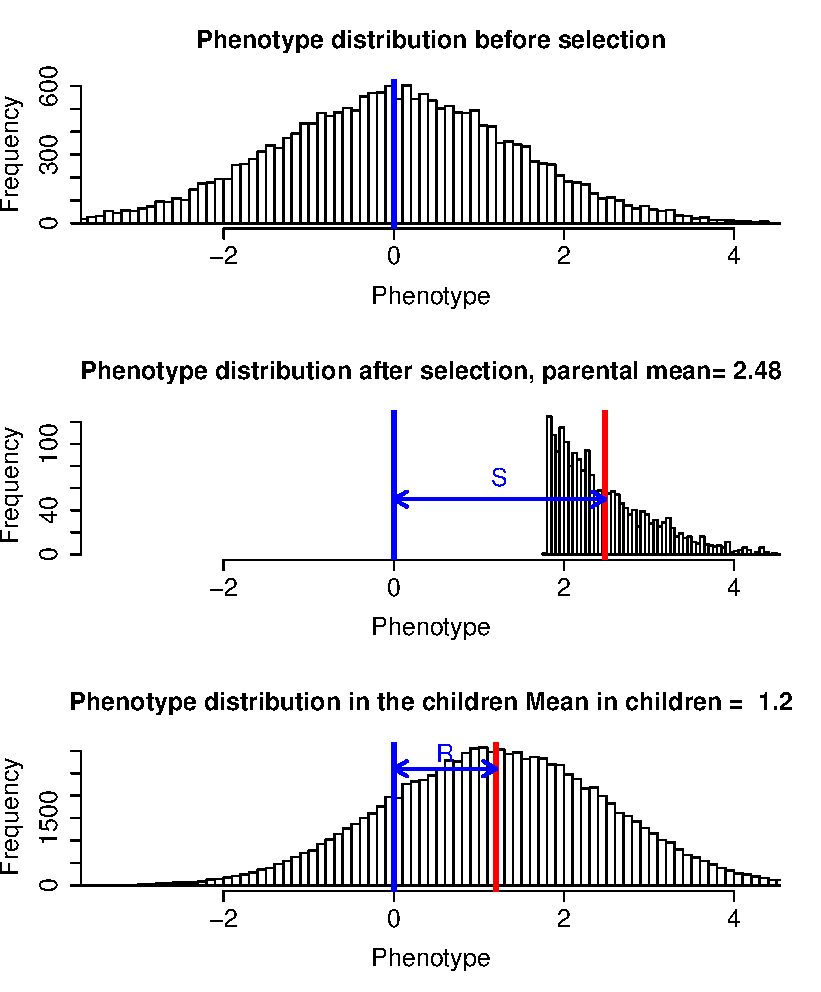
\includegraphics[width=\textwidth]{figures/Response_to_sel/QT3.pdf}
\end{center}
\caption{{\bf Top.} Distribution of a phenotype in the parental population
  prior to selection, $V_A=V_E=1$. {\bf Middle.} Only individuals in the top $10\%$
  of the phenotypic distribution are selected to reproduce; the resulting shift
  in the phenotypic mean is $S$. {\bf Bottom.}  Phenotypic distribution of
  children of the selected parents; the shift in the mean phenotype is
$R. $}
\end{marginfigure}

We are interested in predicting the distribution of phenotypes in the next
generation. In particular, we are interested in the mean phenotype in
the next generation to understand how directional selection has
contributed to evolutionary change. We'll denote the mean phenotype in
offspring, i.e. the mean phenotype in the next generation before selection acts,
as $\mu_{NG}$. The change across generations we'll call the response
to selection $R$ and put this equal to $\mu_{NG}- \mu_{BS}$. \\


The mean phenotype in the next generation is
\begin{equation}
\mu_{NG} = \E \left( \E(X_{kid} | X_{mum},X_{dad}) \right)
\end{equation}
where the outer expectation is over possible pairs of randomly mating individuals
who survive to reproduce. We can use eqn. \ref{predict_kid} to obtain
an expression for this expectation:
\begin{equation}
\mu_{NG} = \mu_{BS} +
\beta_{mid,kid} ( \E(X_{mid}) - \mu_{BS})
\end{equation}

\begin{marginfigure}
\begin{center}
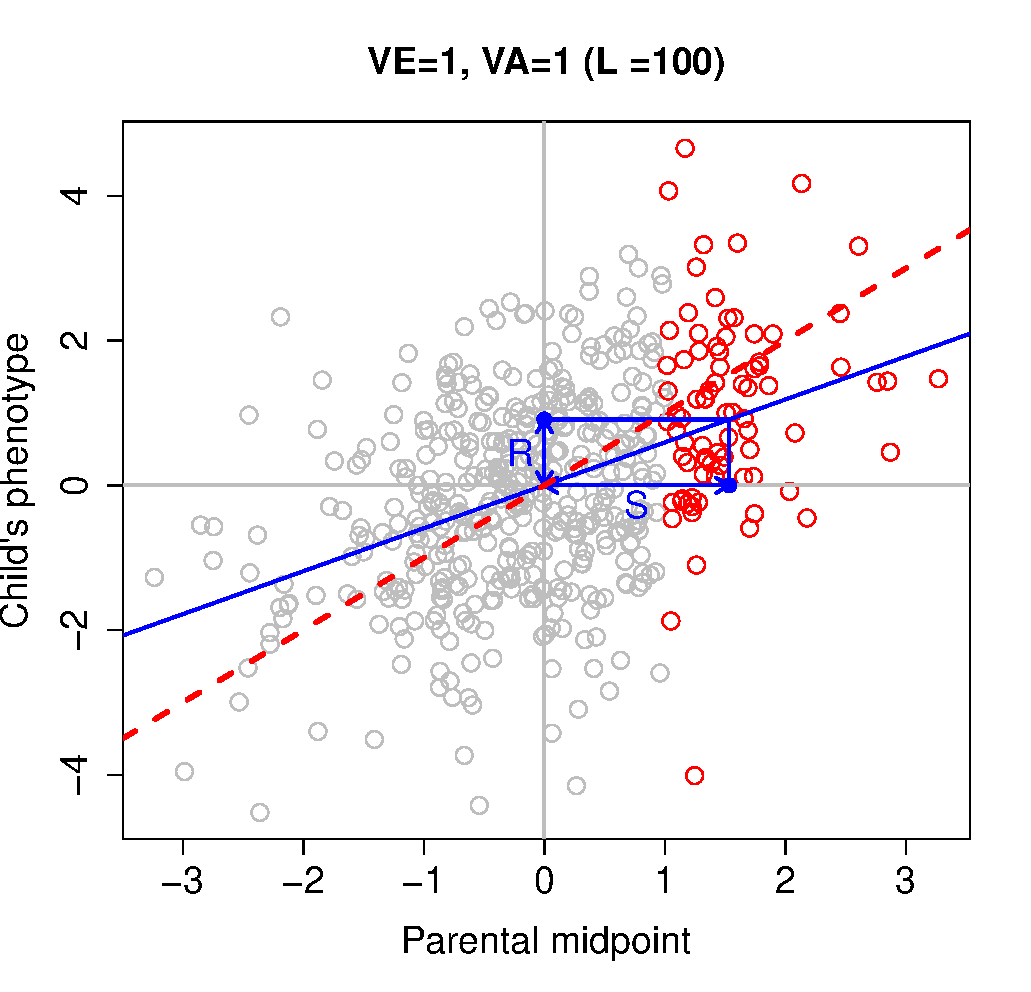
\includegraphics[width=\textwidth]{figures/Response_to_sel/Breeders_eqn.pdf}
\end{center}
\caption{A visual representation of the Breeder's equation. Regression of child's phenotype on parental mid-point phenotype ($V_A=V_E=1$). Under truncation selection, only individuals
  with phenotypes $>1$ (red) are bred.}
\end{marginfigure}

So to obtain $\mu_{NG}$ we need to compute $\E(X_{mid})$, the expected
mid-point phenotype of pairs of individuals who survive to
reproduce. Well this is just the expected phenotype in the individuals
who survived to reproduce ($\mu_{S}$), so
\begin{equation}
\mu_{NG} = \mu_{BS} +
h^2 (\mu_S - \mu_{BS})
\end{equation}
So we can write our response to selection as
\begin{equation}
R = \mu_{NG} -\mu_{BS}  =
h^2 (\mu_S - \mu_{BS}) = h^2 S \label{breeders_eqn}
\end{equation}
So our response to selection is proportional to our selection
differential, and the constant of proportionality is the narrow sense
heritability. This equation is sometimes termed the Breeder's
equation. It is a statement that the evolutionary change across
generations ($R$) is proportional to the change caused by directional selection
within a generation ($S$), and that the strength of this relationship is
determined by the narrow sense heritability ($h^2$). \\

%\graham{Lost the barncle question, put it back in.}



\begin{figure}
\begin{center}
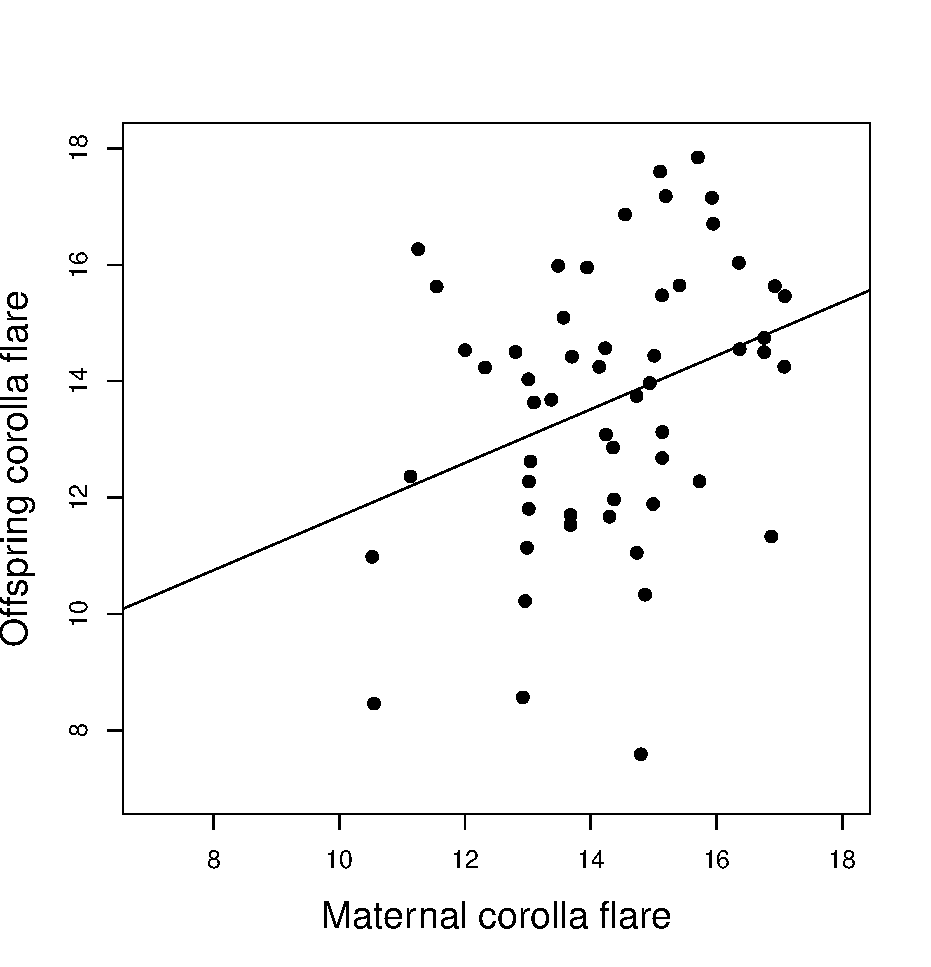
\includegraphics[width= 0.6 \textwidth]{Journal_figs/Quant_gen/Galen_flower_herit/Galen_corolla_flare.pdf} 
\end{center}
\caption{The relationship between maternal and offspring corolla flare (flower
  width) in P. viscosum. Data from \citet{galen:96}. From \citeauthor{galen:96}'s data the covariance of mother and child is 1.3, while the variance of the mother is 2.8.} \label{fig:Galen_corolla}  
\end{figure}

\begin{marginfigure}
\begin{center}
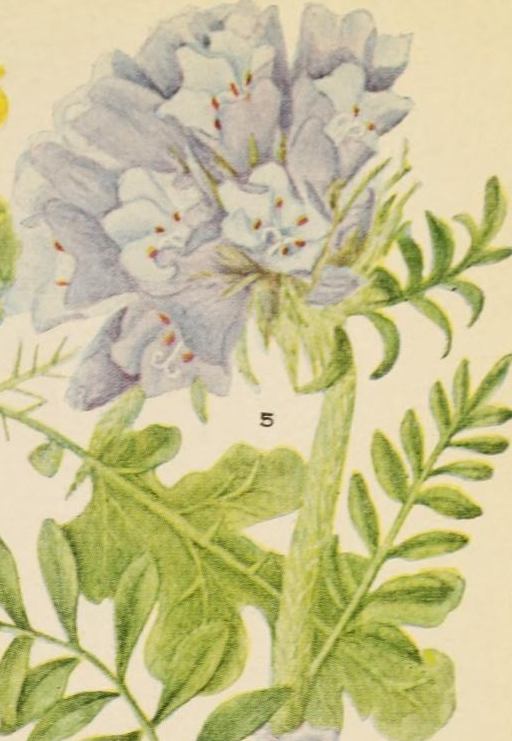
\includegraphics[width=0.75\textwidth]{illustration_images/Quant_gen/Polemonium_viscosum_Galen/Polemonium_viscosum.jpg}
\end{center}
\caption{{\it Plemonium viscosum.}  Modified from Flowers of Mountain and Plain. New York :H.W. Wilson Co.,1920. \href{https://www.flickr.com/photos/biodivlibrary/8220461305/in/album-72157632108046380/}{BHL}. }
\end{marginfigure}


\begin{question}
\citet{galen:96} explored selection on flower shape in
{\it P. viscosum}.  She found that plants with larger corolla flare
had more bumblebee visits, which resulted in higher seed set and a
$17\%$ increase in corolla flare in the plants contributing to the
next generation. Based on the data in Fig. \ref{fig:Galen_corolla}
what is the expected response in the next generation?
\end{question}




\paragraph{The long-term response to selection}
If our selection pressure is sustained over many generations, we can
use our breeder's equation to predict the response. If we are willing
to assume that our heritability does not change and we maintain a constant selection
gradient, then after $n$ generations our phenotype mean will have
shifted 
\begin{equation}
n h^2 S
\end{equation}
i.e. our population will keep up a linear response to selection.

\begin{question}
A population of red deer were trapped on Jersey (an island off of
England) during the last inter-glacial period. From the fossil record \cite{lister:89}
we can see that the population rapidly adapted to their new
conditions. Within 6,000 years they evolved from an estimated mean weight of
the population of 200kg to an estimated mean weight of 36kg (a 6 fold
reduction)! You estimate that the generation time
of red deer is 5 years and, from a current day population, that the narrow sense heritability of the
phenotype is 0.5.\\
{\bf A)}	Estimate the mean change per generation in the mean body weight. \\

{\bf B)}	Estimate the change in mean body weight caused by
selection within a generation. State your assumptions.\\

{\bf C)}	Assuming we only have fossils from the founding population and the population after 6000 years, should we assume that the calculations accurately reflect what actually occurred within our population?
\end{question}


\paragraph{Alternative formulations of the Breeder's equation.}
A change in mean phenotype within a generation occurs because of the
differential fitness of our organisms. To think more carefully about this change within a
generation, let's think about a simple fitness model where our phenotype affects the
viability of our organisms (i.e. the probability they survive to
reproduce). The probability that an individual has a phenotype $X$
before selection is $p(X)$, so that the mean phenotype before
selection is
\begin{equation}
\mu_{BS} = \E[X] =  \int_{-\infty}^{\infty} x p(x) dx
\end{equation}
The probability that an organism with a phenotype $X$ survives to
reproduce is $w(X)$, and we'll think about this as the fitness of
our organism. The probability distribution of phenotypes in those who
do survive to reproduce is
\begin{equation}
\P(X | \textrm{survive}) =  \frac{p(x) w(x)}{
\int_{-\infty}^{\infty} p(x) w(x) dx}.
\end{equation}
where the denominator is a normalization constant which ensures that
our phenotypic distribution integrates to one. The denominator also
has the interpretation of being the mean fitness of the population,
which we'll call $\wbar$, i.e.  
\begin{equation}
\wbar =  
\int_{-\infty}^{\infty} p(x) w(x) dx.
\end{equation}


Therefore, we can write the mean phenotype in those who survive to
reproduce as
\begin{equation}
\mu_S = \frac{1}{\wbar}\int_{-\infty}^{\infty} x p(x) w(x) dx
\end{equation}

If we mean center our population, i.e. set the phenotype before
selection to zero, then
\begin{equation}
S= \frac{1}{\wbar}\int_{-\infty}^{\infty} x p(x) w(x) dx
\end{equation}
%if $\mu_S=0$. \erin{do you mean $\mu_{BS}=0$?} 
Inspecting this more closely, we can see that $S$ has
the form of a covariance between our phenotype $X$ and our fitness
$w(X)$ ($S = Cov(X, w(X))$). Thus our change in mean phenotype is directly a measure of the
covariance of our phenotype and our fitness. Rewriting our breeder's
equation using this observation we see
\begin{equation}
R = \frac{V_A}{V}  Cov(X,w(X))
\end{equation}
we see that the response to selection is due to the fact that our
fitness (viability) of our organisms/parents covaries with our phenotype, and
that our child's phenotype is correlated with our parent's phenotype. 

The phenotype-fitness covariance divided by the phenotypic variance, $Cov(X,w(X))/ V$, is the slope of the linear regression of phenotype on fitness. Let's call this slope the fitness gradient and denote it by $\beta$. Then, equivalently, we can write the breeder's equation as
\begin{equation}
R= V_A \beta
\end{equation}
i.e. we'll see a directional response to selection if there is a linear relationship of phenotype on fitness, and if there is additive genetic variance for the phenotype. 

As one example of a fitness gradient, in Figure \ref{fig:red_deer_fitness_grad}  the lifetime reproductive success (LRS) of male Red Deer is plotted against the weight of their antlers. The red line gives the linear regression of fitness (LRS) on antler mass and the slope of this line is the fitness gradient ($\beta$). 

\begin{marginfigure}
\begin{center}
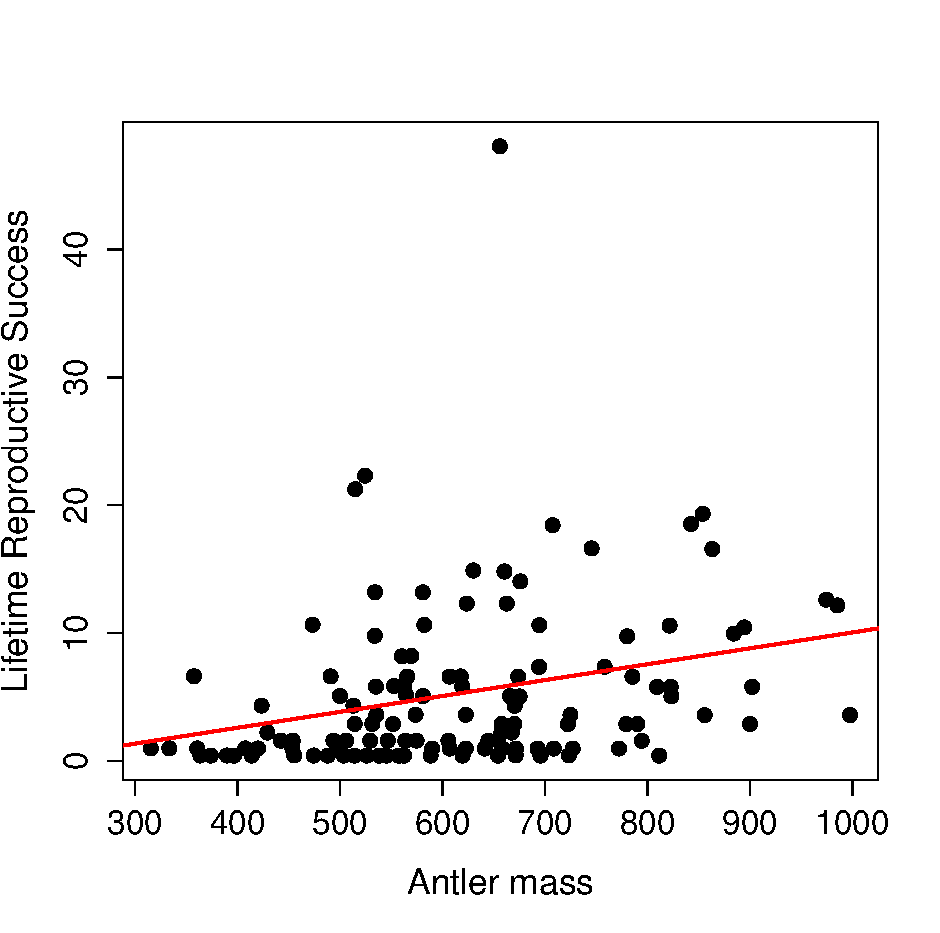
\includegraphics[width= \textwidth]{Journal_figs/Quant_gen/red_deer_selection_gradient/selection_grad_deer.pdf}
\end{center}
\caption{Lifetime reproductive success (LRS) of male Red Deer as a function of their antler mass. } \label{fig:red_deer_fitness_grad}  
\end{marginfigure}

\subsection{The response of multiple traits to selection, the
  multivariate breeder's equation.}
We can generalize these results for multiple traits, to ask how selection on
multiple phenotypes plays out over short time intervals. \cite{lande:79} Considering two traits we can write our responses in both traits as
\begin{eqnarray}
R_1 & = V_{A,1} \beta_1 + V_{A,1,2} \beta_2 \nonumber \\
R_2 & = V_{A,2} \beta_2 + V_{A,1,2} \beta_1  \nonumber \\
\end{eqnarray}
where the $1$ and $2$ index our two different traits. Here $V_{A,1,2}$ is our additive covariance between our traits. Our selection gradient for trait 1, $\beta_1$, represents the change in fitness changing trait 1 alone holding everything else constant. This is a statement that our response in any one phenotype is modified by selection on other traits that covary with that trait. This offers a good way to think about how genetic trade offs play out over short-term evolution.

We can also write this in matrix form. We can write
our change in the mean of our multiple phenotypes within a generation as the vector $\bf{S}$ and our response across multiple generations as
the vector $\bf{R}$. These two quantities are related by 
\begin{equation}
\bf{R} = \bf{G} \bf{V}^{-1} \bf{S} = \bf{G} \boldsymbol{ \beta}
\end{equation}
 where $\bf{V}$ and $\bf{G}$ are our matrices of the
 variance-covariance of phenotypes and additive genetic values
 (eqn. \eqref{G_matrix} \eqref{P_matrix}) and
 $\boldsymbol{\beta}$ is a vector of selection gradients (i.e. the change within a generation as a fraction of the total phenotypic variance). 

\begin{question}
You collect observations of red deer within a generation, recording an
individual's number of offspring and phenotypes for a number of traits which are known to
have additive genetic variation. Using your data, you construct the plots shown in
Figure \ref{fig:red_deer_Q} (standardizing the phenotypes). Answer the following
questions by choosing one of the bold options. Briefly justify each of your answers with reference to the breeder's
equation and multi-trait breeder's equation. \\
{\bf A)}	Looking just at figure \ref{fig:red_deer_Q} A, in what direction do you expect male antler size to evolve? \\
{\bf Insufficient information, increase, decrease.}\\

{\bf B)}	Looking just at figures \ref{fig:red_deer_Q} B and C, in what direction do you expect male antler size to evolve? \\
{\bf Insufficient information, increase, decrease.}\\

{\bf C)}	Looking at figures \ref{fig:red_deer_Q} A, B, and C, in what direction do you expect male antler size to evolve? \\
{\bf Insufficient information, increase, decrease.}\\
\end{question}

\begin{figure}
\begin{center}
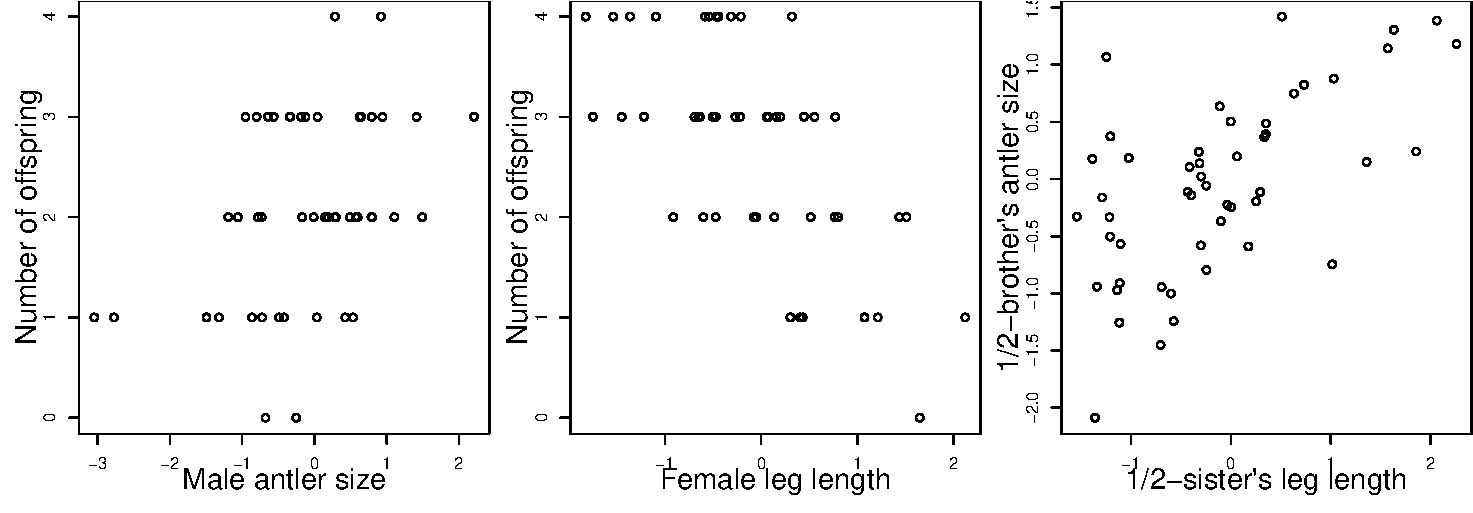
\includegraphics[width=\textwidth]{figures/Red_deer_selection.pdf}
\end{center}
\caption{ Observations of red deer within a generation; recording an
individual's number of offspring and phenotypes (simulated data), which are known to
have additive genetic variation. The figures left to right are A-C.  } \label{fig:red_deer_Q}
\end{figure}



As an example of correlated responses to selection, consider the  \citeauthor{wilkinson:93} selection experiment on Stalk-eyed
 flies ({\it Cyrtodiopsis  dalmanni}). Stalk-eyed flies have evolved amazingly long eye-stalks. In the lab, \citeauthor{wilkinson:93} established six populations of
 wild-caught flies and selected up and down on males eye-stalk to body
 size ratio for 10 generations (left plot in Figure
 \ref{fig:Stalk_eyed_response}). Despite the fact that he did not
 select on females, he saw a correlated response in the females from
 each of the lines (right plot), because of the genetic correlation
 between male and female body proportions. 

\begin{figure}
\begin{center}
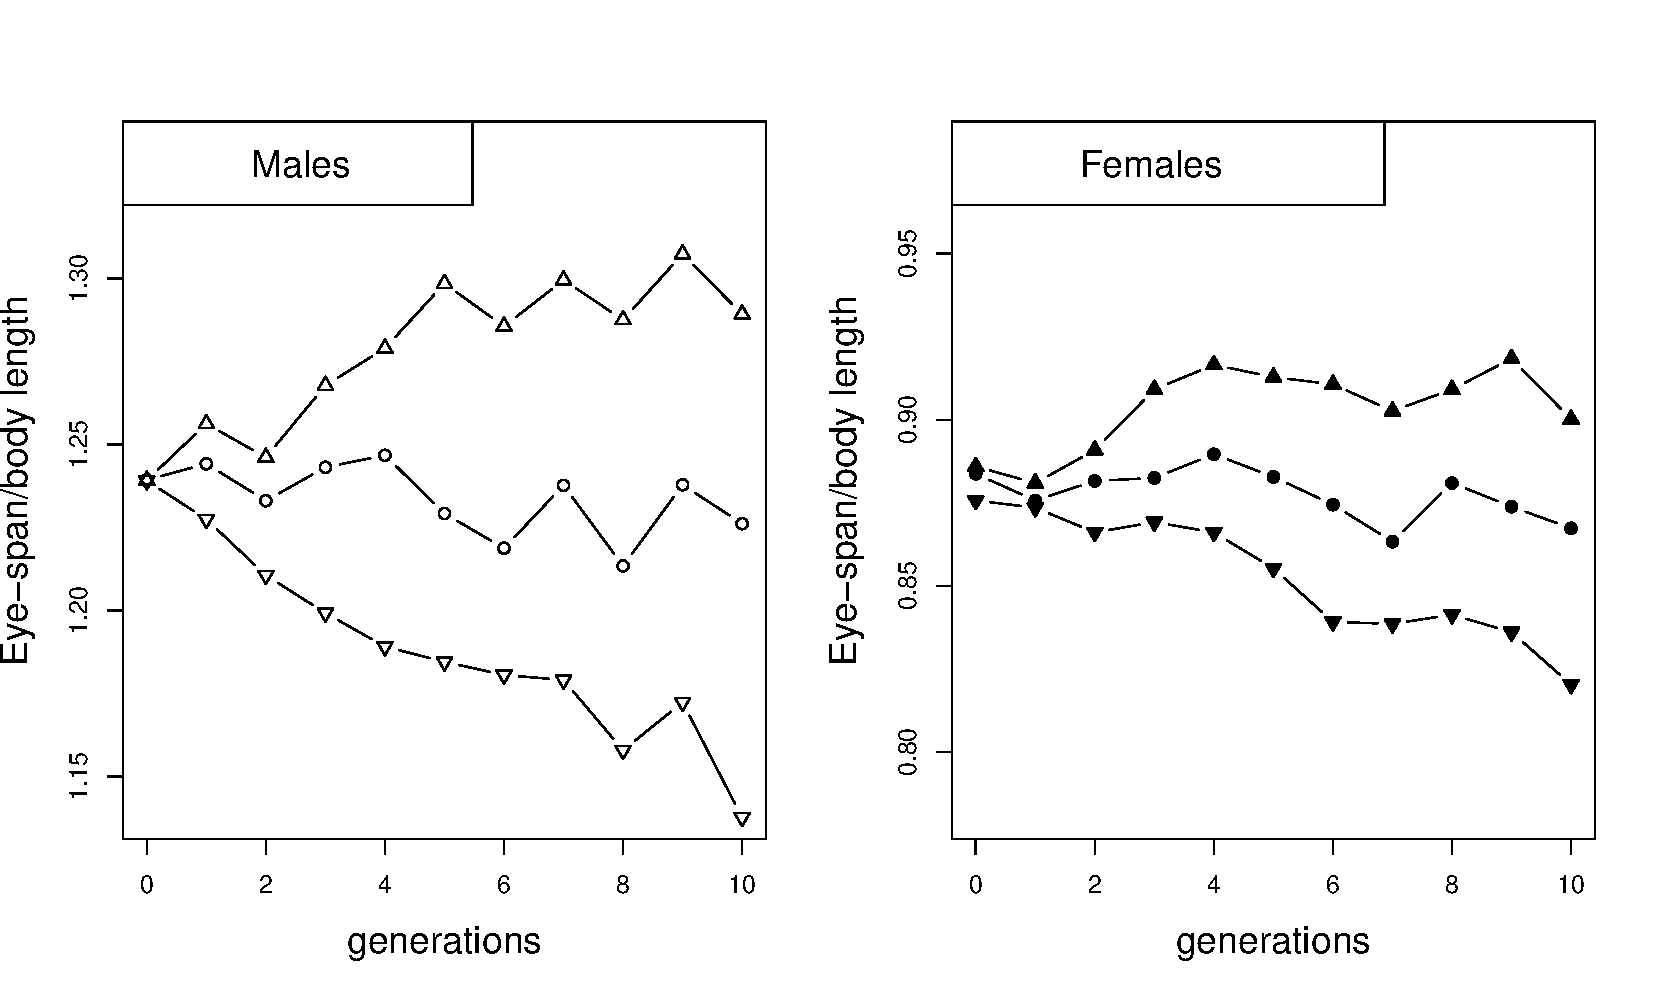
\includegraphics[width= \textwidth]{Journal_figs/Quant_gen/stalk_eyed_flies/stalk_eyed_flies_response.pdf}
\end{center}
\caption[][-1cm]{ \citeauthor{wilkinson:93} selected two of populations for flies for
 increased and eye-stalk to body length ratio in males (mean shown as
 up triangles), and two for a
 decreased ratio (down triangles), by taking the top 10 males with the highest (lowest)
 ratio out of 50 measures. He also established two control populations
 (circles). He constructed each generation of females by sampling 10
 at random from each population.  

} \label{fig:Stalk_eyed_response}   %\cite{potti:11} 
\end{figure}

\begin{marginfigure}[1cm]
\begin{center}
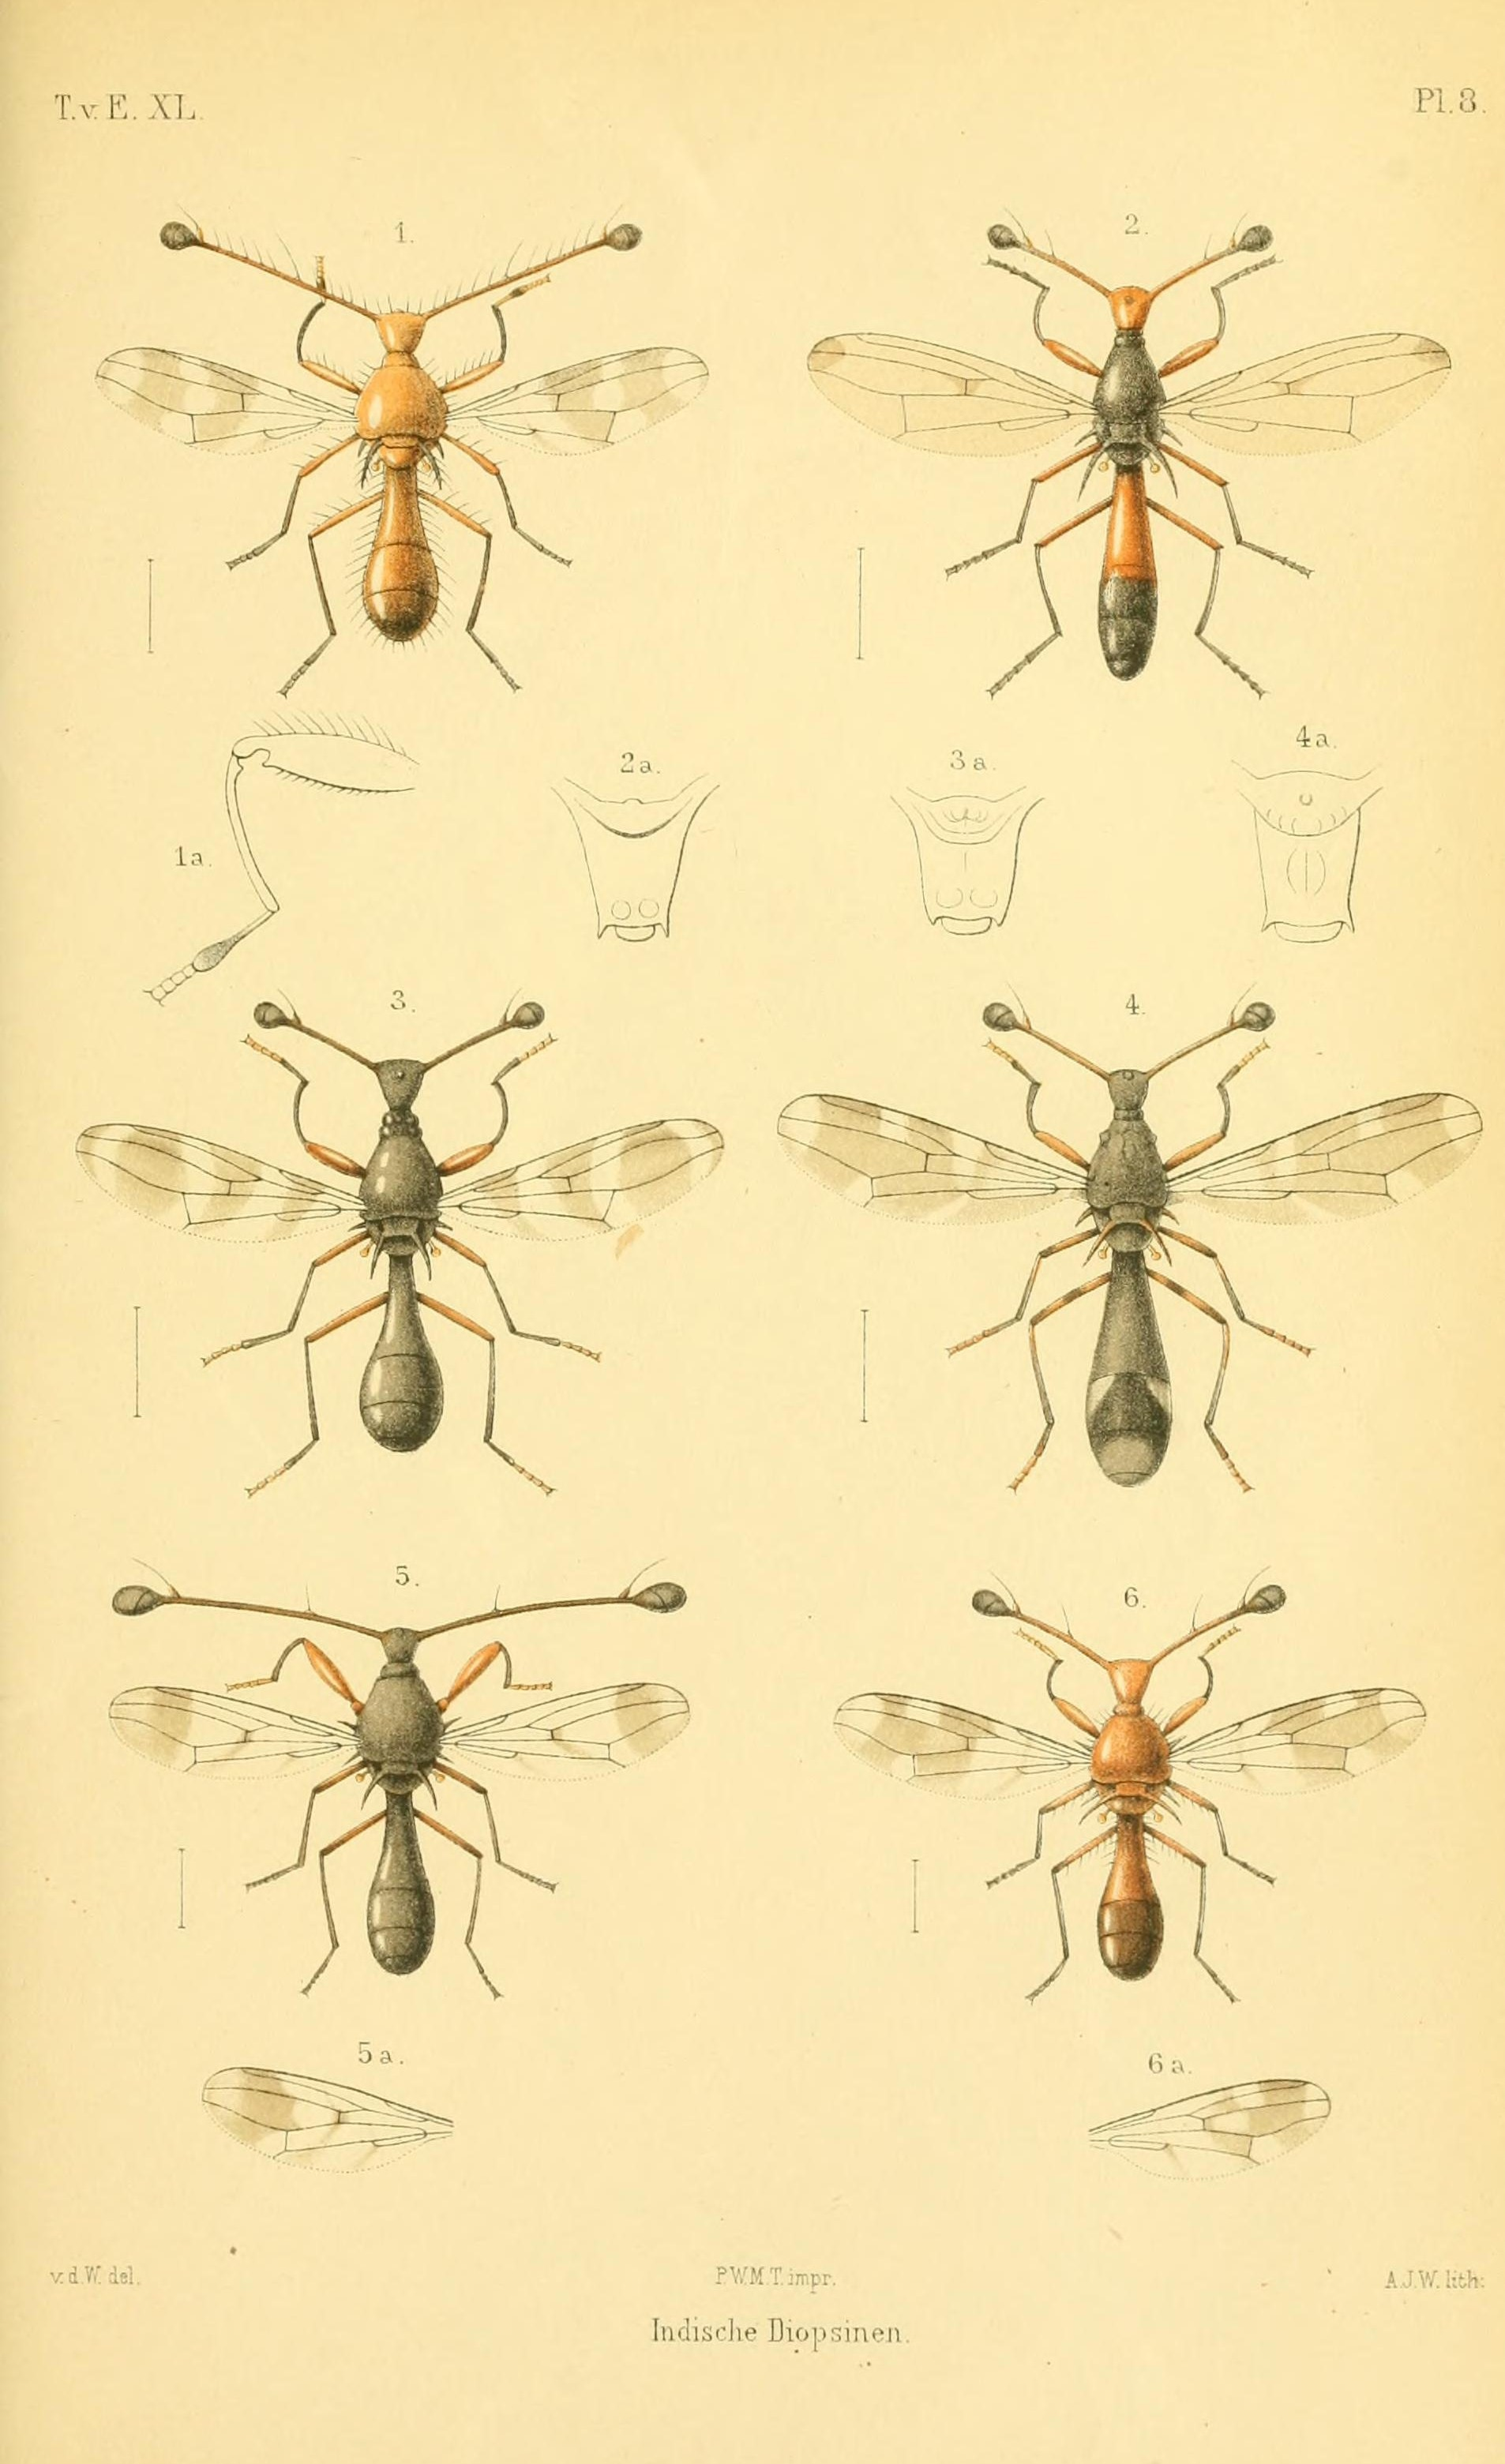
\includegraphics[width=0.9 \textwidth]{illustration_images/Quant_gen/Stalk_eyed_flies/WulpPlateVIIIjpg.jpg}
\end{center}
\caption{Stalk-eyed Flies ({\it Diopsidae}).  Diptera.
van der Wulp. 1898. BHL} \label{fig:Stalk_eyed_flies}  
\end{marginfigure}
\begin{question}

At the end of ten generations in \citeauthor{wilkinson:93}'s experiment (Figure
\ref{fig:Stalk_eyed_response}), the males from the up- and down-selected
lines had mean eye-stalk to body ratios of $1.29$ and $1.14$
respectively, while the females from the up- and down-selected lines
had means of $0.9$ and $0.82$. \\
{\bf A)} \citeauthor{wilkinson:93} estimated that by selecting the top/bottom 10 males, he had on average shifted the mean body ratio by 0.024 within
each generation. What is the male heritability of eye-stalk to body-length ratio?

{\bf B)} Assume that the additive genetic variance of male and female phenotypes are
equal and that there is no direct
selection on female body-proportion in this experiment, i.e. that all of
the response in females is due to correlated selection. Can you
estimate the male-female genetic correlation of the eye-stalk ratio? 
\end{question}




\section{Some applications of the multivariate trait breeder's equation}

The multivariate breeders equation has a lot of different uses in understanding the response of multiple traits to selection. It also offers some insights into kin selection and sexual selection. We'll discuss these next.

\paragraph{Hamiliton's Rule and the evolution of altruistic and selfish behaviours}


Individuals frequently behave in ways that sacrifice their own fitness for the
benefit of others. That selection favours such apparent acts of altruism is puzzling at first site. \citet{hamilton1964genetical,hamilton1964genetical2} supplied the first general evolutionary explanation of such altruism.
His intuition was that while an individual is losing
out of some reproductive output, the alleles underlying an altruistic behaviour
can still spread in the population if this cost is outweighed by benefits gained 
through the transmission of these alleles through a related individual (note that this means that the
allele is not acting in an self-sacrificing manner, even though
individuals may as a result). 
We can use our quantitative genetics framework to gain some simple
intuition for when altruistic behaviours should evolve through kin
selection. To do this, we can derive a simple version of Hamilton's
Rule by thinking about the phenotypes of an individual's kin as
genetically correlated phenotypes.

To do this, we
can follow a simplified \citet{queller1992quantitative} treatment, to re-derive Hamilton's rule in a quantitative genetics framework (Hamilton's original work did this in a
population genetics framework).

Altruism reflects social interactions. So as a simple model let's imagine that individuals interact in pairs, with our focal
individual $i$ being paired with an individual $j$.  
Imagine that individuals have two possible phenotypes $X=1$ or $0$,
corresponding to providing or withholding some small act of `Altruism'
(we could just as easily flip these labels and call them an unselfish
act and a selfish act respectively). 
Our pairs of individuals interacting could, for example, be siblings sharing a
nest. The altruistic trait could be as simple as growing at a
slightly slower rate so as to reducing sibling-competition for food from
parents, or more complicated acts of altruism such as foregoing their
own reproduction so as to help their parents raise their siblings.

Providing the altruistic act has a cost $C$ to the fitness of our
individual and failing to provide this act has no cost. Receiving this
altruistic act confers a fitness benefit $B$ (not receiving it has no benefit).
Hamiliton's rule states that such a trait will spread through the
population if the average coefficient of relatedness between the
interaction individuals is $r$, the average number of alleles that
our pairs of individuals share identical by descent at a locus. We can express
Hamilton's rule as
\begin{equation}
 C<rB
\end{equation}

\begin{marginfigure}
\begin{center}
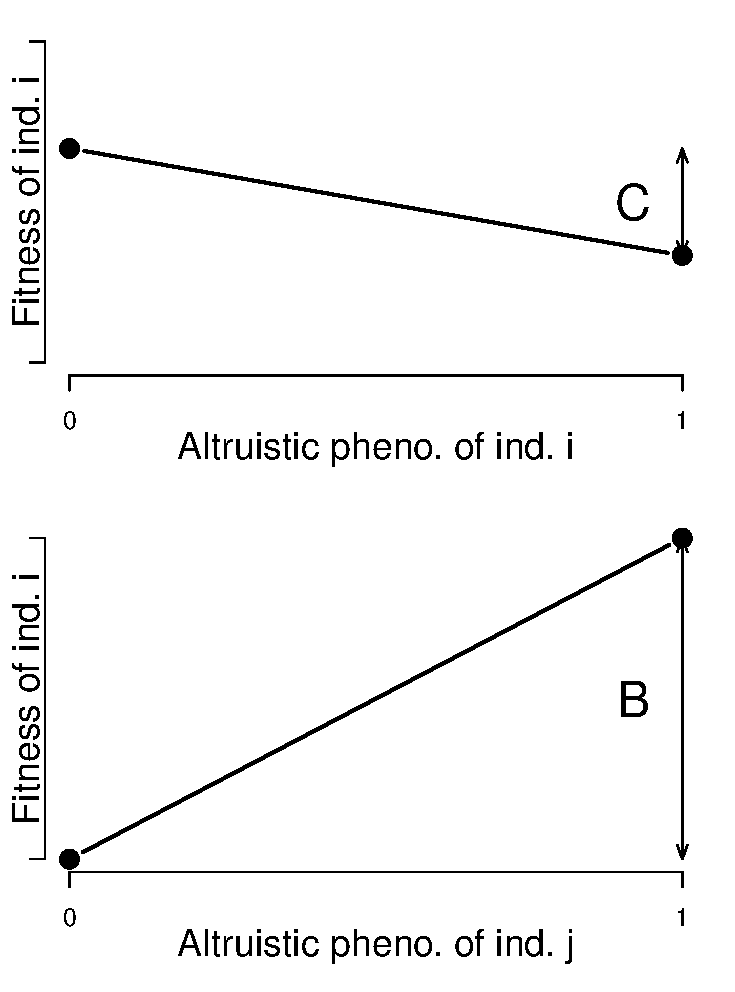
\includegraphics[width= \textwidth]{figures/Response_to_sel/Hamiltons_rule_B_C.pdf}
\end{center}
\caption{ } \label{fig:Hamilton_B_C}
\end{marginfigure}



To sketch a proof of this result, let's assume that our focal $i$ individual's relative fitness can be written as 
\begin{equation}
W(i,j)= W_0 + W_i +W_j
\end{equation}
where $W_i$ is the contribution of the fitness of the individual $i$ due
to their own phenotype, and $W_j$ is the contribution to our
individual $i$'s fitness due to the interacting individual $j$'s behaviour (i.e. phenotype).
With the benefit $B$ and cost $C$, our $W(i,j)$ are depicted in
Figure \ref{fig:Hamilton_B_C}. 

We can write the expected change in phenotype as 
\begin{equation}
R = \beta_i V_A + \beta_j V_{A,i,j}
\end{equation}
Our altruistic phenotype is increasing in the population if $R>0$,
i.e. if
\begin{eqnarray}
  \beta_i V_A + \beta_j V_{A,i,j} > 0  \nonumber  \\
& \beta_j \frac{V_{A,i,j}}{V_A}  > -\beta_i 
\end{eqnarray}
So what's the average genetic covariance between
individual $i$ and $j$'s alturistic phenotype? Well the covariance of
the same phenotype between two individuals is just $2 F_{i,j} V_A$ (see \eqref{additive_covar_general_rellys}). Our $F_{i,j}$ is the probability that an allele found in individual
$i$ is identical by descent to an allele drawn from individual $j$. Therefore $2 F_{i,j}$
can be interpreted as the average number of alleles shared between
individuals $i$ and $j$. So 
\begin{eqnarray}
 -\beta_i < & \beta_j \frac{2 F_{i,j} V_A}{V_A} \nonumber  \\
-\beta_i < & \beta_j 2 F_{i,j} \nonumber  \\
C < & r  B \\
\end{eqnarray}


\paragraph{Sexual selection and the evolution of mate preference by indirect benefits. }

Organisms often put an enormous effort into attracting mates, sometimes at
a considerable cost to their chances of survival. 

One major reason why individuals are choosy about who they mate with is
that it can directly impact their fitness. By choosing a mate with
particular characteristics, individuals can gain more parental care for
their offspring, avoid parasites, or be choosing a mate with higher
fertility. However, even in the absence of direct benefits, selection
can still indirectly favour the evolution of choosiness. These
indirect benefits occur because individuals can have higher fitness
offspring by choosing a mate whose phenotype indicates high viability
(the so-called good genes hypothesis), or by \ec{choosing a mate whose phenotype is simply attractive, and likely to produce similarly attractive offspring (the sexy sons hypothesis).} \erin{I attempted to finish this sentence for you .. it just ended partway through}

We'll denote a display trait, e.g. tail length, in males by $\mars$ and a preference
trait in females by $\venus$. Our display trait is under direct selection in males, such that its response to selection can be written as
\begin{equation}
R_{\mars} = \beta_{\mars} V_{A, \mars}
\end{equation}
Let's assume that the female preference trait, the degree to which
females are attracted to long tails, is not under direct
selection $\beta_{\venus}=0$. Then the response to selection of the
preference trait can be written as
\begin{eqnarray}
R_{\venus} &=\beta_{\venus}V_{A,\venus}  + \beta_{\mars} V_{A, \venus
  \mars}
& = \beta_{\mars} V_{A, \venus  \mars}
\end{eqnarray}
So the female preference will respond to selection if it is
genetically correlated with the male trait, i.e. if $V_{A, \venus
  \mars}$ \ec{is not zero}. There's a number of different ways this genetic correlation could arise; the
simplest is that the loci underlying the male trait may have a
pleiotropic effect on female preference. However, female preference
may often have quite a distinct genetic basis from male display traits.

A more general way in which trait-preference genetic correlations may
arise is through assortative mating. As females vary in their
tail-length preference, the ones with a preference for longer
tails will mate with long-tailed males and the opposite for females
with a preference for shorter-tails. Therefore, a
genetic correlation between mates display and preference traits will
become established (see Figure \ref{fig:assort_mating_2_trait}). 
\begin{figure}
\begin{center}
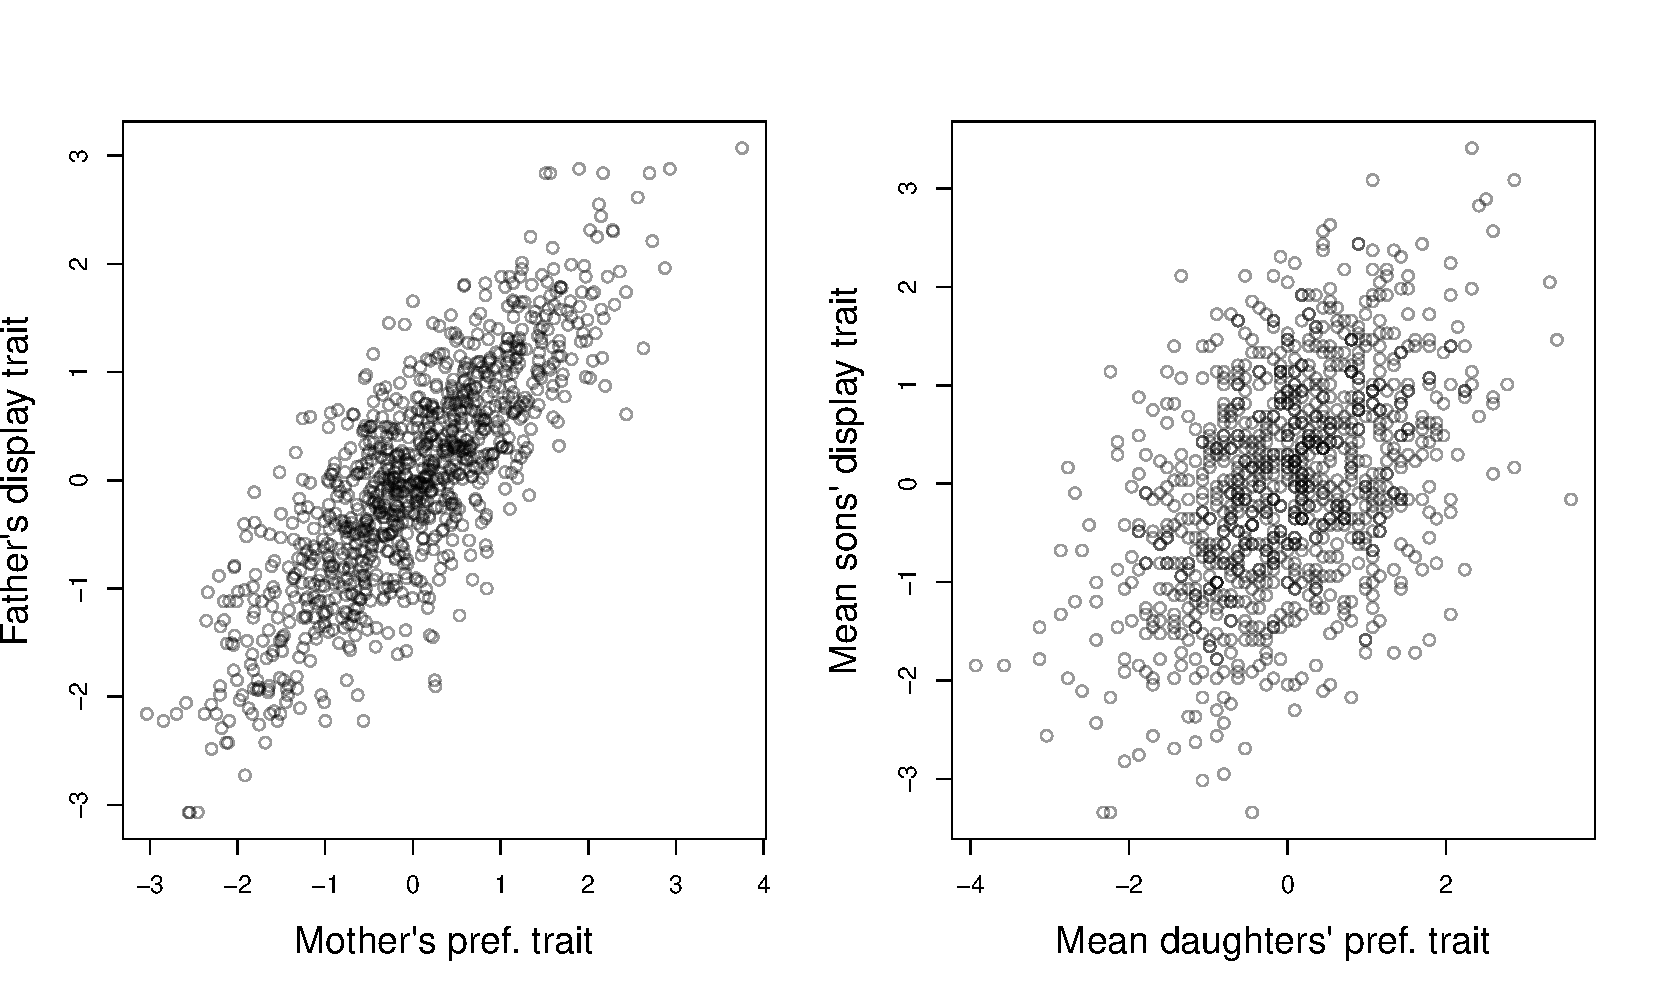
\includegraphics[width=\textwidth]{figures/Response_to_sel/Genetic_corr_assort_mating.pdf}
\end{center} \label{fig:assort_mating_2_trait}
\caption{}
\end{figure}
The males with the longer tails will also carry the alleles
associated with the preference for longer tails, as their long-tailed
dads tended to mate with females with a genetic preference for long
tails. Similarly, the the males with shorter tails will carry alleles associated with the preference for
shorter tails. Thus if there is direct selection for males with longer tails, then
the female preference for longer tails will increase too, as it is
genetically correlated via assortative mating. \erin{I don't take away from this description that you can get runaway sexual selection without external directional selection for longer tails ... can you make that more clear? I think the problem is making the female trait a preference for short vs. long tails when maybe it should be presented as a preference for long tails vs. no preference so the males with longer tails get a boost from positive sexual selection. Also, why do you plot mean daughter's trait against mean son's trait and not, say, mean father's trait against mean daughter's trait or increase in population prevalence or correlation between male-female traits over time?}

As an example of how selection on display traits can drive the
evolution of preference traits, let's consider some data from guppies. Guppies ({\it Poecilia reticulata}) are a classic system for studying
the interplay of natural and sexual selection. In some populations of
guppies, females show a preference for males with more orange colouration. \citeauthor{houde:94} established four replicate population pairs of
guppies ({\it Poecilia reticulata}) and selected one of each pair for
an increased or decreased orange coloration in males, selecting the top/bottom $20$ out of $50$
males. She randomly chose females from each population to form the next generation, and so did not
exert direct selection on females. She measured the response to 
selection on male colouration and on female preference for orange (left
and right panels of Figure \ref{fig:assort_mating_guppies}
respectively). In the lines that were selected for more orange males \erin{this section needs completion}.

\begin{figure}
\begin{center}
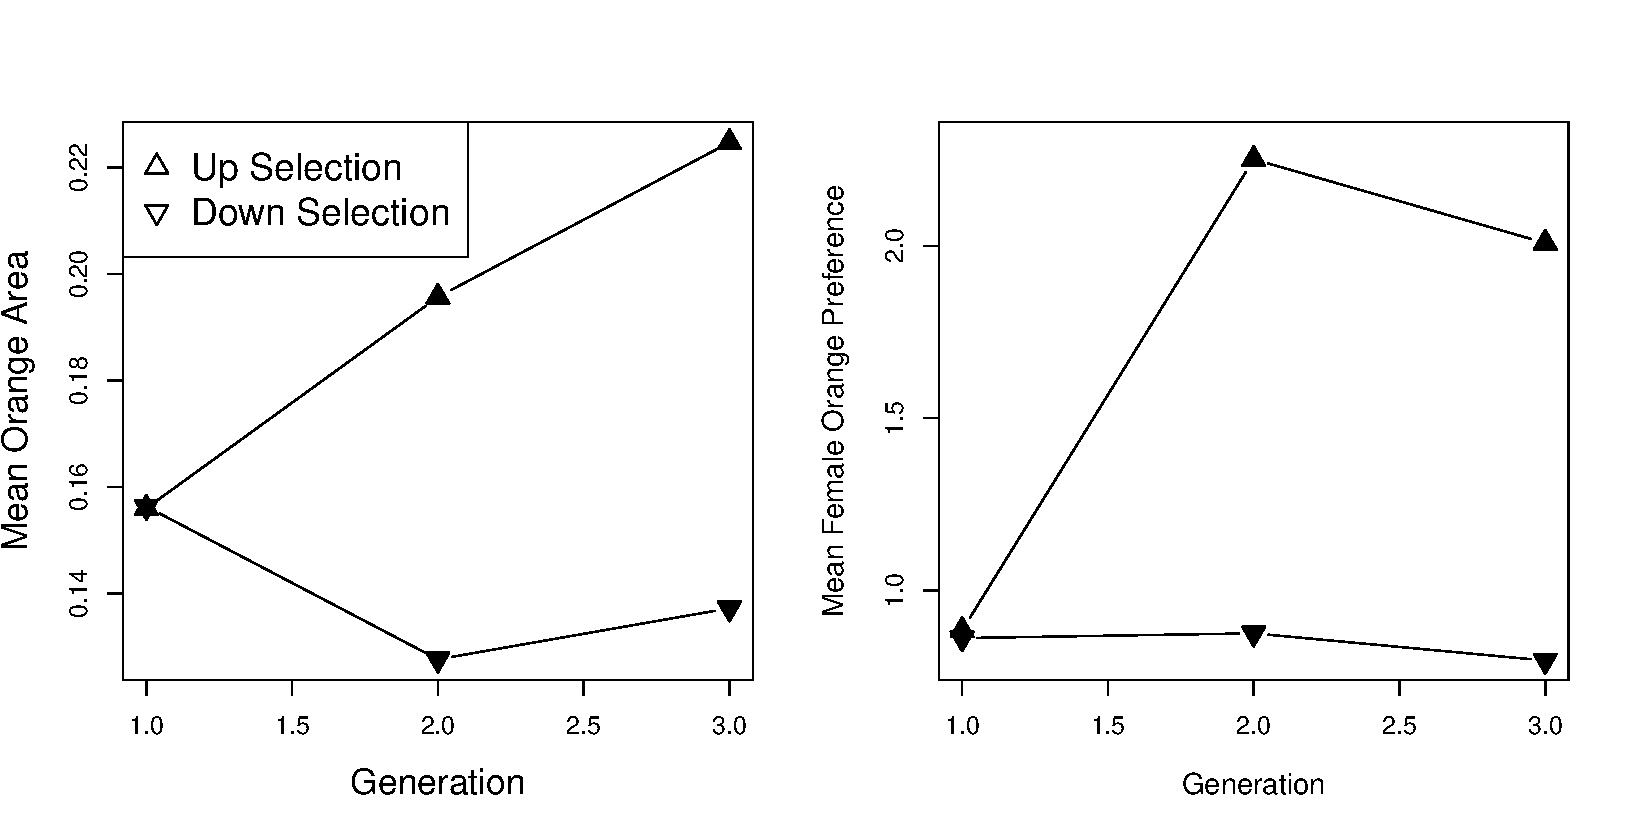
\includegraphics[width=\textwidth]{Journal_figs/Quant_gen/guppies_female_choice/guppies_female_choice.pdf}
\end{center} \label{fig:assort_mating_guppies}
\caption{Mean phenotypes for the two up- and two down-selected
  populations of Guppies. Left panel: A response to selection was seen
  due to the direct selection on male colouration. Right panel: An
  indirect, correlated response was also seen in female preference. Redrawn from \citeauthor{houde:94}.}
\end{figure}

% potential guppy image https://www.google.com/imgres?imgurl=https%3A%2F%2Fc1.staticflickr.com%2F1%2F457%2F20360503816_a88cdcd96d_b.jpg&imgrefurl=https%3A%2F%2Fwww.flickr.com%2Fphotos%2Finternetarchivebookimages%2F20360503816&docid=jtYRcc7UmAvIeM&tbnid=DBAauK0xAgK4mM%3A&vet=10ahUKEwirkrKWy8rcAhWTAHwKHfVdCmUQMwg2KAEwAQ..i&w=1024&h=840&itg=1&client=firefox-b-1-ab&bih=681&biw=1280&q=Lebistes%20reticulatus&ved=0ahUKEwirkrKWy8rcAhWTAHwKHfVdCmUQMwg2KAEwAQ&iact=mrc&uact=8
